\documentclass{beamer}

\usepackage{listings}
\lstset{language={[LaTeX]TeX}, basicstyle=\small}

\usepackage{multimedia}

\usepackage{hyperref}
\usepackage[utf8]{inputenc}
\usepackage{xspace}

\useoutertheme{shadow}
\usecolortheme{beaver}

\newcommand{\singleitem}[1]{\begin{itemize}\item #1\end{itemize}}
\newcommand{\pdfpc}{\texttt{pdfpc}\xspace}
\newcommand{\opt}[1]{\texttt{#1}\xspace}

\setbeamertemplate{navigation symbols}{}

\defbeamertemplate{footline}{my foot}{%
\vskip1pt%
\makebox[0pt][l]{\insertshortauthor}%
\hspace*{\fill}\insertshorttitle\hspace*{\fill}%
\llap{\insertframenumber\phantom{/}}
}
\setbeamertemplate{footline}[my foot]

\mode<presentation>

\title{\pdfpc video demo}
\author[E. Stambulchik]{Written by
                  \href{https://github.com/fnevgeny}{Evgeny Stambulchik}}
\date{\today}
\institute{}

\begin{document}

\begin{frame}
  \titlepage
  \hypertarget{titlePage}{}
\end{frame}

\begin{frame}
  \frametitle{About this demo}

  This file demonstrates support for video playback in \pdfpc.
  Open it with: \opt{pdfpc video-example.pdf}
  
  \vfill
  
  {\small The NASA video from the Apollo 17 mission, used in this demo, is
  in the public domain.}
  
\end{frame}

\begin{frame}
  \frametitle{Two modes of including video media}

  \pdfpc supports two ways of including movies in PDF:

  \begin{itemize}
    \item As the screen annotations;
    \item As the ``launch'' hyperlinks.
  \end{itemize}

  \begin{block}{}
    The first approach is standards-compatible, but currently has a limited
    support for playback options (in part due to third-party software
    limitations). The second solution is more versatile, but is \pdfpc-specific
    (meaning the video playback will work {\em only} in \pdfpc).
  \end{block}

  \begin{alertblock}{}
    It is {\em strongly} recommended to use the standard approach, since the
    ``propriety'' one will likely be removed in the future.
  \end{alertblock}
\end{frame}

\begin{frame}[fragile]
  \frametitle{\opt{multimedia} package}

  The \opt{multimedia} package is a part of \opt{latex-beamer}, but can
  also be used standalone. A minimal code to include a movie would look like
  this:

  \begin{lstlisting}
    \usepackage{multimedia}
    ...
    \movie{\includegraphics{poster.png}}{movie.avi}
  \end{lstlisting}

  \begin{itemize}
    \item Here, ``poster.png'' is the still image that is shown before the movie
      starts playing (usually, it should be its first frame).
    \item Instead of the local movie, a valid URL pointing to a remote video
      file can be passed.
    \item You can adjust the size of the video by passing the usual
      width/height/etc arguments to the {\opt{\textbackslash includegraphics}}
      command.
  \end{itemize}

  \vspace{10pt}
  Switch to the next page to see it in action.
\end{frame}

\begin{frame}
  \frametitle{Example 1}
  \vspace{10pt}
  \begin{center}
    \movie{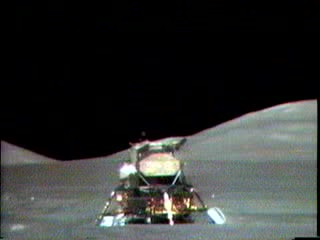
\includegraphics[width=0.7\textwidth]{apollo17.jpg}}{apollo17.avi}
  \end{center}
    
  \begin{itemize}
    \item Click on the image to play/pause the video.
    \item Move pointer to the bottom of the video frame for a draggable position
      control.
  \end{itemize}
\end{frame}

\begin{frame}[fragile]
  \frametitle{\opt{\textbackslash movie} options}
  
  \pdfpc supports a subset of options of the \opt{\textbackslash movie} command:

  \begin{itemize}
    \item \opt{showcontrols} -- always show the position bar control;
    \item \opt{once} -- play the video once and stop (this is the default);
    \item \opt{loop} or \opt{repeat} -- play the video in the loop.
  \end{itemize}
    
  \vspace{20pt}

  E.g., 
  \begin{lstlisting}
    \movie[loop]{\includegraphics{poster}}{movie.avi}
  \end{lstlisting}

  \vspace{10pt}
  Switch to the next page to see it in action.
\end{frame}

\begin{frame}
  \frametitle{Example 2}

  \vspace{10pt}
  \begin{center}
    \movie[loop]{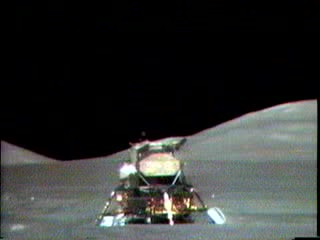
\includegraphics[width=0.7\textwidth]{apollo17}}{apollo17.avi}
  \end{center}

  \singleitem{Once started, this video will play back in the loop}

\end{frame}

\begin{frame}
  \frametitle{Subtitles}

  \pdfpc has a basic support for subtitles. 
  
  \vspace{10pt}

  To enable, it must be invoked with the \opt{-T} option. Then for each video
  played back, \pdfpc will try to load a subtitle file (in the SRT format) by
  appending ``.srt'' to its path (or URL).
  
  \singleitem{There is also a respective \opt{pdfpcrc} option if you want to
    make this the default behavior}
\end{frame}

\begin{frame}[fragile]
  \frametitle{The non-standard method}

  If you {\em desperately} need a finer control of the movie playback, consider
  using the \opt{\textbackslash href\{run:\}} hack.

  The syntax is like

  \begin{lstlisting}
    \usepackage{hyperref}
    ...
    \href{run:movie.avi?options}
       {\includegraphics{poster.png}}
  \end{lstlisting}

  Here, the possible ``options'' are
  \begin{itemize}
    \item loop -- infinite loop;
    \item start=n -- start playing at \opt{n} sec from the beginning;
    \item stop=n -- stop the playback at \opt{n} sec from the beginning;
    \item autostart -- start the video once the page is shown;
    \item srtfile=URL -- load a SRT file with subtitles from the given
      location.
  \end{itemize}

\end{frame}

\begin{frame}
  \frametitle{Example 3}

  An example using the \opt{\textbackslash href\{run:\}} hack. The
  video is set to automatically start playing in the loop a fragment of the
  movie between 5 seconds and 12 seconds from the beginning.

  \vspace{5pt}

  \begin{center}
    \href{run:apollo17.avi?autostart&loop&start=5&stop=12}
       {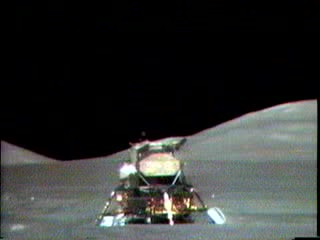
\includegraphics[height=0.7\textheight]{apollo17.jpg}}
  \end{center}
\end{frame}

\begin{frame}
  \frametitle{The end}
  
  As always, refer to the \opt{pdfpc(1)} and \opt{pdfpcrc(5)} man pages.

\end{frame}

\end{document}
